%%%%%%%%%%%%%%%%%%%%%%%%%%%%%%%%%%%%%%%%%%%%%%%%%%%%%%%%%%%%%%%%%
% Contents: Main Input File of the LaTeX2e Introduction
% $Id: lshort-base.tex 447 2010-12-14 14:32:00Z oetiker $
%%%%%%%%%%%%%%%%%%%%%%%%%%%%%%%%%%%%%%%%%%%%%%%%%%%%%%%%%%%%%%%%%
% lshort.tex - The not so short introduction to LaTeX
%                                                      by Tobias Oetiker
%                                                     oetiker@ee.ethz.ch
%
%                           based on LKURTZ.TEX Uni Graz & TU Wien, 1987
%-----------------------------------------------------------------------
%
% To compile lshort, you need TeX 3.x, LaTeX and makeindex
%
% The sources files of the Intro are:
%      lshort.tex (this file),
%      titel.tex, contrib.tex, biblio.tex
%      things.tex, typeset.tex, math.tex, lssym.tex, spec.tex,
%      lshort.sty, fancyheadings.sty
%
% Further the  verbatim.sty and the layout.sty
% from the LaTeX Tools distribution is
% required.
%
%
% To print the AMS symbols you need the AMS fonts and the packages
% amsfonts, eufrak and eucal from (AMS LaTeX 1.2)
%
% ---------------------------------------------------------------------

%%%%%%%%%%%%%%%%%%%%%%%%%%%%%%%%%%%%%%%%%%%%%%%%%%%%%%%%%%%%%%%%%
% Contents: Who contributed to this Document
% $Id: contrib.tex 533 2015-04-09 13:00:40Z oetiker $
%%%%%%%%%%%%%%%%%%%%%%%%%%%%%%%%%%%%%%%%%%%%%%%%%%%%%%%%%%%%%%%%%
\begin{small}
  \noindent Copyright \copyright 2014-2015 Lianhua Zhu.  All rights reserved.

  This document is free; you can redistribute it and/or modify it
  under the terms of the GNU General Public License as published by
  the Free Software Foundation; either version 2 of the License, or
  (at your option) any later version.
  This document is distributed in the hope that it will be useful, but
  \emph{without any warranty}; without even the implied warranty of
  \emph{merchantability} or \emph{fitness for a particular purpose}\@.  See the GNU
  General Public License for more details.
  You should have received a copy of the GNU General Public License
  along with this document; if not, write to the Free Software
  Foundation, Inc., 675 Mass Ave, Cambridge, MA 02139, USA.
\end{small}


\pagebreak
\endinput
%

% Local Variables:
% TeX-master: "dugksFoam"
% mode: latex
% mode: flyspell
% End:

%%%%%%%%%%%%%%%%%%%%%%%%%%%%%%%%%%%%%%%%%%%%%%%%%%%%%%%%%%%%%%%%%
% Contents: Who contributed to this Document
% $Id: overview.tex 456 2011-04-06 09:10:27Z oetiker $
%%%%%%%%%%%%%%%%%%%%%%%%%%%%%%%%%%%%%%%%%%%%%%%%%%%%%%%%%%%%%%%%%

% Because this introduction is the reader's first impression, I have
% edited very heavily to try to clarify and economize the language.
% I hope you do not mind! I always try to ask "is this word needed?"
% in my own writing but I don't want to impose my style on you...
% but here I think it may be more important than the rest of the book.
% --baron

\chapter{Preface}

The dugksFoam is an OpenFOAM solver for the Boltzmann equation with the Shakhov collision model.
The numerical method behind it is the discrete unified gas kinetic scheme (DUGKS, see Ref.~\cite{guozl15}).
The DUGKS discretizes the governing equation in both physical space and velocity space.
It solves the partial differential equations of the discrete velocity distribution functions in a finite volume framework.
In DUGKS, the fluxes of distribution functions are constructed from the local characteristic solution of the governing equation itself.
This feature makes DUGKS very efficient for simulating near continuum flows.

The OpenFOAM is one of the most popular open-source general CFD toolkits.
The biggest feature of it is that it allows users to develop their own solvers in a very high level.
The OpenFOAM provides the solver developers varies ready-to-use major components of numerical solving of PDE (mainly for finite-volume discretization),
such as the arbitrary unstructured mesh representation, spatial discretization operator, time integration schemes,
boundary condition types and message passing interface (MPI) based parallelization.
In the development of a typical OpenFOAM solver,
the developer spends most of the time to define the solving procedure,
i.e., writing the Field Operation And Manipulation expressions.
Besides these basic components, OpenFOAM also provides a branch of general utilities for pre-processing,
post-processing, parallel computing, job control etc.

By implementing the DUGKS into an OpenFOAM solver, we can take many advantages of the OpenFOAM toolkit.
Such as the easy pre and post processing, parallelization, solving control and parameter configurations.
We expect it can be a convenient tool for study non-equilibrium gas flow and heat transfer problem in complex geometries.
In addition, it can serve as a reference for developing other kinetic type equations such as the phonon transport equation, semiconductor equation etc.,
because solving kinetic type equation in OpenFOAM is not so that common compared with those macro-filed based solvers the OpenFOAM provides.
The only kinetic type equation solver appears in official OpenFOAM distribution is the discrete ordinates model (DOM) for thermal radiation computation.

In this documentation, we present the installation, usages, demo cases of the dugksFoam.
For the detailed information about the DUGKS, one can refer to the papers by Guo et al\cite{guozl13,guozl15}.
For the detailed of implementation of the DUGKS in unstructured mesh and the configuration of demo cases in this documentation,
one can refer the paper post on arxiv.org by the author\cite{zhulh15}.

\endinput
%

% Local Variables:
% TeX-master: "lshort2e"
% mode: latex
% mode: flyspell
% End:

\tableofcontents
%\listoffigures
%\listoftables
\enlargethispage{\baselineskip}
\mainmatter
%%%%%%%%%%%%%%%%%%%%%%%%%%%%%%%%%%%%%%%%%%%%%%%%%%%%%%%%%%%%%%%%%
% Contents: Things you need to know
% $Id: things.tex 536 2015-06-26 06:41:33Z oetiker $
%%%%%%%%%%%%%%%%%%%%%%%%%%%%%%%%%%%%%%%%%%%%%%%%%%%%%%%%%%%%%%%%%

\chapter{Installation}

\label{inst}
Before the installation of dugksFoam, you should have installed the OpenFOAM together with the ThirdParty tools on your Linux machine.
The download address of OpenFOAM and the detailed installation instructions can found in the
\href{http://openfoam.org/download/}{official web site of OpenFOAM} and the ~\href{https://openfoamwiki.net/index.php/Main_Page}{OpenFOAM wiki}.
The OpenFOAM versions I have tested is 2.2.1, 2.3.0 and 2.4.0.
But the dugksFoam should also works on the latest release of OpenFOAM (Ver.~3.0.0 or above).

The detailed installation instructions are as follows.
\begin{enumerate}
\item Load the OpenFOAM environment:
Type the command \texttt{ofxxx} where \texttt{xxx} is the three digits of the OpenFOAM version you installed,
if you have followed the official installation instructions of OpenFOAM. For example, \texttt{of240} or \texttt{of230}.
\item Create your own solvers installation location, and cd to it :
\begin{verbatim}
mkdir -p $FOAM_RUN/../applications
cd $FOAM_RUN/../applications
\end{verbatim}
\item Get the source code using git (see below) from \href{https://github.com/zhulianhua/dugksFoam}{dugksFoam repository}
or download it as a ZIP package by clicking \href{https://github.com/zhulianhua/dugksFoam/archive/master.zip}{here}.
\begin{itemize}
\item If using git:
\begin{verbatim}
git clone git@github.com:zhulianhua/dugksFoam.git
cd dugksFoam/src
\end{verbatim}
\item If installing by ZIP package, move the ZIP package (\texttt{dugksFoam-master.zip}) to \verb|$FOAM_RUN/../applications|. Then unzip it by
\begin{verbatim}
unzip dugksFoam-master.zip
mv dugksFoam-master dugksFoam
cd dugksFoam/src
\end{verbatim}
\end{itemize}

\item For OpenFOAM release older than 2.4.0, there is a compatible issue in the make file options about \verb|meshTool|.
If you are using OpenFOAM older than 2.4.0, fix it by this command:
\begin{verbatim}
git apply PatchMeshToolIssue
\end{verbatim}

\item Compile the dugksFoam by:
\begin{verbatim}
./Allwmake
\end{verbatim}

\item Check if the compilation is OK:
\begin{verbatim}
which dugksFoam
\end{verbatim}
It should tell you where the compiled executable \verb|dugksFoam| is.
\end{enumerate}
%

% Local Variables:
% TeX-master: "dugksFoam"
% mode: latex
% mode: flyspell
% End:



%

% Local Variables:
% TeX-master: "dugksFoam"
% mode: latex
% mode: flyspell
% End:
\chapter{Usage}

\section{Overview}

Besides the standard \texttt{system/controlDict}, the mesh files in \verb|constant/polyMesh| and the initial fields (\verb|0| directory),
you should also provide the following additional configuration files,
\begin{itemize}
\item \verb|constant/Xis| : the discrete velocity set in 1D;
\item \verb|constant/weights| : the weight coefficients corresponding to the discrete velocity set;
\item \verb|constant/DVMparameters| : sets the gas parameters and discrete velocity information;
\item \verb|system/fvSchemes| : sets the discrete scheme for the gradient evaluation.
\item \verb|system/fvSolution| : dummy file (sets nothing).
\end{itemize}
The formats for these configuration files are described in the following subsections.
It is recommoned to always start a new case by copy-and-modifying an existing case, such as the the demo cases provided with the dugksFoam source code (see Sec.~\ref{sec_cavity}).

\section{Step by step guide}
\subsection{Prepare the physical meshes}
Generate the mesh either by using \verb|blockMesh/snappyHexMesh| provided by OpenFOAM or using a third party mesh generation softwares,
such as Gambit, pointwise, ICEM CFD or gmsh.
Note that some of the third party softwares in recent release support exporting mesh files in OpenFOAM internal format directly, such as the pointwise.
Nevertheless, you can always convert a mesh in other formats into a OpenFOAM internal format by the mesh-conversing tools provided by OpenFOAM,
such as the \verb|fluentMeshToFoam| or \verb|gmshToFoam|.

I personally use the Gambit a lot. The general procedure is :
\begin{enumerate}
\item Build the geometry and meshing it in Gambit.
\item Export fluent mesh file in Gambit, say \verb|demo.msh|.
\item Copy the fluent mesh (\verb|demo.msh|) to your case directory.
\item Convert the fluent mesh to OpenFOAM mesh by
\begin{verbatim}
fluentMeshToFoam demo.msh
\end{verbatim}
\end{enumerate}
\subsection{Set initial macro variable field and boundary conditions}
The initial macro field files in the \verb|0| directory required are,
\begin{itemize}
\item \verb|0/rho| : the initial density field;
\item \verb|0/U|   : the initial velocity field;
\item \verb|0/T|   : the initial temperature field.
\end{itemize}
Set the initial values (usually uniform) for the three macro fields.
Modify the boundary condition types for each boundary patch in the three files according to the physical boundary condition types.
The solver supports several commonly seen physical boundary condition types. There are
\begin{itemize}
\item diffusive wall boundary;
\item specular reflection wall boundary
\item far field boundary;
\end{itemize}
Their usages are presented in the following.
\subsubsection{Diffusive wall boundary}
For the diffusive wall boundary, you need to set the corresponding boundary patch in \verb|0/rho| to \verb|calculatedMaxwell| together with a dummy uniform value.
Below is an example:
\begin{verbatim}
    boundaryField
    {
         ...
         topWall
         {
              type            calculatedMaxwell;
              value           uniform 1.0;
         }
         ...
    }
\end{verbatim}
You should also set the corresponding boundary patch in \verb|0/U| and \verb|0/T| as \verb|fixedValue| type and provide the wall's moving velocity and temperature.

\subsubsection{Specular reflection wall boundary (symmetric boundary)}
Physically, the specular reflection wall boundary is identical to the symmetry boundary.
Currently, the dugksFoam supports only symmetry boundaries aligned in the X/Y/Z directions.
To specify a symmetric boundary, set the corresponding boundary patch type as \verb|symmetryPlane| in all of the three initial fields, i.e., \verb|0/rho|, \verb|0/U|, \verb|0/T|.
Note that you should also change the basic boundary patch type in \verb|constant/polyMesh/boundary| to \verb|symmetryPlane|.

\subsubsection{Far field boundary}
This boundary type is exclusively used for the outer boundary in the simulation of supersonic extern flows past objects.
The physical interpretation is that the particles comes into the computational domain with the far field equilibrium velocity distribution.
To specify such a boundary type, just set the boundary types as \verb|fixedValue|, and provide the free-stream flow condition as the boundary values in
\verb|0/rho|, \verb|0/U| and \verb|0/T|.

\subsection{Prepare the discrete velocity set}
\label{sec_dv}
The dugksFoam currently only support Cartesian grids in velocity space.
And the grid points are identical in each direction for 2D or 3D problems, i.e., $\xi_{ix} = \xi_{iy} = \xi_{iz} \equiv \xi_i$.
For 1D and 2D problems, it uses the dimensional reduction technique in the velocity space, which improves its efficiency considerably.
The discrete velocity set $\xi_i$ and the corresponding weights $w_i$ are provided by two files,
the \verb|constant/Xis| and \verb|constant/weights|. Each of the files represents a 1D list.
Below are examples of \verb|constant/Xis| and \verb|constant/weights| files corresponding to a 28 point discrete velocity grid.

\begin{itemize}
\item \verb|constant/Xis|:
\begin{verbatim}
    FoamFile
    {
        version     2.0;
        format      ascii;
        class       scalarList;
        location    "constant";
        object      Xis;
    }
    // ********************************************* //
    28
    (
    -1.7664856627356885e+03
    -1.5149431219611315e+03
    -1.3067831284809952e+03
     //...
     //... skip of 22 lines
     //...
     1.3067831284809952e+03
     1.5149431219611315e+03
     1.7664856627356885e+03
    );
    // ********************************************* //
\end{verbatim}

\item \verb|constant/weights|:
\begin{verbatim}
    FoamFile
    {
        version     2.0;
        format      ascii;
        class       scalarList;
        location    "constant";
        object      weights;
    }
    // ********************************************* //
    28
    (
     2.9037294321023950e+02
     2.2430119141828482e+02
     1.9483915929202675e+02
     //...
     //... skip of 22 lines
     //...
     1.9483915929202675e+02
     2.2430119141828482e+02
     2.9037294321023950e+02
    );
    // ********************************************* //
\end{verbatim}
\end{itemize}
For Newton-Cotes quadrature and half-range Gauss-Hermite quadrature,
we provide the script \verb|setDV.py| to modify the two files conveniently.
The script is located in \verb|src/scripts|.
If you followed the installation steps in Sec.~\ref{inst},
you should be able to run \verb|setDv.py| and thus set those files directly.
For example, to set a 28-points Gauss-Hermite discrete velocity set, simply run
\begin{verbatim}
    setDV.py GH 408.16 28
\end{verbatim}
where \verb|GH| stands for Gauss-Hermite,  \verb|408.16| is the most probable molecular speed,
and \verb|28| is the number of discrete velocities.
Or to set a 81-points compound Newton-Cotes rule discrete velocity set, run
\begin{verbatim}
    setDV.py NC 2000.0 81
\end{verbatim}
where \verb|NC| stands for Newton-Cotes, \verb|2000.0| stands for the max discrete velocity, and \verb|81| is  the number of discrete velocities
\subsection{Set gradient evaluation schemes}
There are two schemes available to evaluate the gradients of distribution during the reconstruction step.
They are \verb|leastSquares| and \verb|Gauss linear|.
Both of them can be modified with a limiter function by the keyword \verb|cellLimited|.
The strength of the limiter can be controlled by a scalar parameter $s,~0 < s < 1$.
$s=0$ means don't limit, while $s=1$ means full limiting.
These options are input in the section of \verb|gradSchemes| of the file \verb|system/fvSchemes|. Below is an example.
Note that \verb|divSchemes| and \verb|laplacianSchemes| are always set to \verb|none| as dugksFoam doesn't use those operators.
\begin{verbatim}
    FoamFile
    {
        version     2.0;
        format      ascii;
        class       dictionary;
        location    "system";
        object      fvSchemes;
    }
    // ********************************************* //
    gradSchemes
    {
        default         leastSquares;
    //  default         cellLimited Gauss linear 1.0;
    //  default         cellLimited leastSquares 0.5;
    }

    divSchemes
    {
        default         none;
    }

    laplacianSchemes
    {
        default         none;
    }
    // ********************************************* //
\end{verbatim}

\subsection{The dummy  fvSolution file}
The  \verb|system/fvSolution| should always be provided as follows
\begin{verbatim}
    FoamFile
    {
        version     2.0;
        format      ascii;
        class       dictionary;
        location    "system";
        object      fvSolution;
    }
    // ********************************************* //
    solvers
    {
    }
    // ********************************************* //
\end{verbatim}
Nothing is set in that file, since the dugksFoam is an explicit solver.

\subsection{Set solving control parameters}
The main control parameters for the solver running, such as when to stop, how often to dump immediate macro fields, time step size etc.\
are set in the file \verb|system/controlDict| as like other OpenFOAM solvers.
Note that you can turn on the \verb|adjustTimeStep| option and provide a maximal CFL number by the \verb|maxCo| keyword. Below is an example of
the \verb|system/controlDict| file
\begin{verbatim}
    FoamFile
    {
        version     2.0;
        format      ascii;
        class       dictionary;
        location    "system";
        object      controlDict;
    }
    // ********************************************* //
    application     dugksFoam;
    startFrom       latestTime;
    startTime       0;
    stopAt          endTime;
    endTime         2.0e2;
    deltaT          4.00e-4;
    //writeControl    adjustableRunTime;
    writeControl    timeStep;
    writeInterval   200;
    purgeWrite      0;
    writeFormat     ascii;
    writePrecision  16;
    writeCompression off;
    timeFormat      general;
    timePrecision   9;
    runTimeModifiable true;
    adjustTimeStep  yes;
    maxCo           0.8;
    maxDeltaT       1;
    // ********************************************* //
\end{verbatim}

\subsection{Set gas properties}
The gas properties are set in the \verb|gasProperties| section of file \verb|constant/DVMProperties|.
You should specify the specific gas constant $R$, the viscosity-temperature relation exponent $\omega$,
the reference temperature $T_\text{ref}$, the reference viscosity  $\mu_\text{ref}$ at $T_\text{ref}$,
and the Prandtl number Pr.
Note that you should also provide the maximum and minimum discrete velocity and the number of
discrete velocity in the \verb|fvDVMparas| section of this file.
They should be consistent with \verb|constant/Xis| files.
An example of the \verb|constant/DVMProperties| file is shown below,
\begin{verbatim}
    FoamFile
    {
        version     2.0;
        format      ascii;
        class       dictionary;
        location    "constant";
        object      DVMProperties;
    }
    // ********************************************* //

    fvDVMparas
    {
        xiMax       xiMax [0 1 -1 0 0 0 0]  2.138251518302359e+03;
        xiMin       xiMin [0 1 -1 0 0 0 0] -2.138251518302359e+03;
        nDV               28;  // Number of discrete velocity
    }

    gasProperties
    {
        R            R [0 2 -2 -1 0 0 0] 208.244343891;
        omega        0.81; // VHS viscosity ~ Temperature index
        Tref         Tref [0 0 0 1 0 0 0] 400.0;
        muRef        muRef [1 -1 -1 0 0 0 0] 1.94014016536e-05;
        Pr           0.666666666666667; // Prantl number
    }
    // ********************************************* //
\end{verbatim}

\subsection{Run in serial or parallel}
If all of the files and parameters described in the previous subsections are prepared, you can finally run the \verb|dugksFoam| solver.
To run \verb|dugksFoam| serially,
\begin{verbatim}
    dugksFoam
\end{verbatim}
To run \verb|dugksFoam| in parallel with \verb|mpirun|, you should firstly decompose the computational domain use the tool \verb|decomposePar|.
Refer the OpenFOAM official User'S Guide to see how.
After the domain decomposition, you can run \verb|dugksFoam| in parallel by
\begin{verbatim}
    mpirun  -np 8 dugksFoam -parallel
\end{verbatim}
where 8 means to use MPI processes.
\subsection{Post processing}
After running the solver, you can see the immediate results directories.
If you run in parallel, you have to reconstruct the results files by \verb|reconstructPar| first.
To view the results, you can use either ParaView or Tecplot.
\begin{itemize}
\item To use ParaView : create an empty file in the case directory by
\begin{verbatim}
    touch a.foam
\end{verbatim}
Then use the ParaView to read the \verb|a.foam|.
\item To use Tecplot : use the tool \href{https://openfoamwiki.net/index.php/FoamToTecplot360}{FoamToTecplot360} to convert the results to Tecplot format results, then use Tecplot.
 Or use the latest releases of Tecplot360 which support reading the OpenFOAM result files directly.
\end{itemize}
\chapter{Demo cases}
\section{2D cavity flow at $\text{Kn}=0.075$}
\label{sec_cavity}
This demonstrational case is provided in the \verb|demos| subdirectory of the dugksFoam source code package.
This case is a popular benchmark problem for validating numerical method for micro or rarefied gas flows.
It has been studied in Ref.~\cite{zhulh15} using this solver,
where you can find the detailed description of this problem.
We only mention some setting that need special attention for a new user.
The mesh file and setting have already been prepared in the case directory.
So you can run the dugksFoam directly.

The flow configuration is illustrated in Fig.~\ref{ldc}.
The walls are diffusive boundaries.
For such a simple geometry, you can use the \verb|blockMesh| shipped with the OpenFOAM to generate the structured mesh.
Refer to the cavity flow tenurial case in the \emph{OpenFOAM User's Guide} for the detailed usage of \verb|blockMesh|.
The initial temperautre filed is uniform 273K, and the wall temperature is also 273K.
In this case, the Knudsen number Kn is 0.075 based on the initial density filed and the cavity width $L$.
So the mean free path is 0.075m.
The initial density field input in the \verb|0/rho| file should be calculated from the mean free path provided the argon gas properties.
Refer to ~\cite{zhulhA} for the related formulations.
We also provide a simple Python script named \verb|para.py| in the case's directory to compute the related parameters.
You can run it by \verb|python para.py|.


The discrete velocities used are $28\times28$ half-range Gauss-Hermite quadrature points.
The files \verb|constant/Xis| and \verb|constant/weights| can be generated by
\begin{verbatim}
    setDV.py GH 337.196399395 28
\end{verbatim}
where 28 is the number of discrete velocity in each direction, and 337.196399395 stands for the most probable speed of argon gas molecular at $T=273$K.
Refer to Sec.~\ref{sec_dv} for more details about settings of discrete velocities.

Fig.~\ref{ldc_UT} show some of the results of this case.
You can also compare the results with those in \cite{lhzhuA} in detail.

\begin{figure}
  \centering
  % Requires \usepackage{graphicx}
  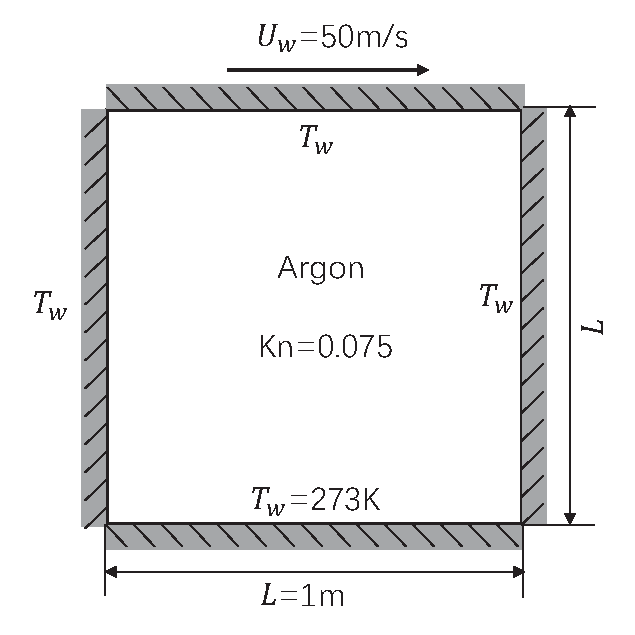
\includegraphics[width=0.4\textwidth]{img/ldc.eps}\\
  \caption{Lid-driven cavity flow}\label{ldc}
\end{figure}

\begin{figure}[htbp]
\centering
\subfloat[]{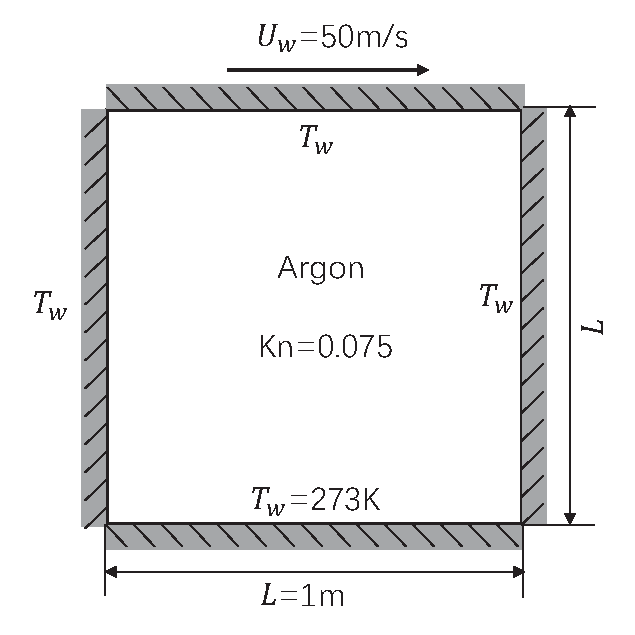
\includegraphics[width=0.48\textwidth]{img/ldc.eps}} ~
\subfloat[]{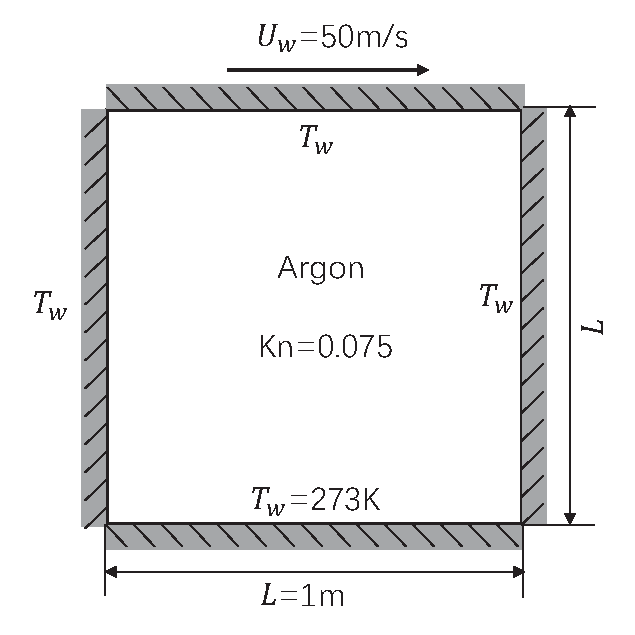
\includegraphics[width=0.48\textwidth]{img/ldc.eps}}
\caption{
Results of the cavity flow case. (a) Temperature contours and heat flux. (b) Velocity magnitude and streamlines.
}\label{ldc_UT}
\end{figure}

% Local Variables:
% TeX-master: "dugksFoam"
% mode: latex
% mode: flyspell
% End:

\backmatter
%%%%%%%%%%%%%%%%%%%%%%%%%%%%%%%%%%%%%%%%%%%%%%%%%%%%%%%%%%%%%%%%%
% Contents: The Bibliography
% File: biblio.tex (lshort2e.tex)
% $Id: biblio.tex 449 2010-12-14 16:53:51Z oetiker $
%%%%%%%%%%%%%%%%%%%%%%%%%%%%%%%%%%%%%%%%%%%%%%%%%%%%%%%%%%%%%%%%%
\begin{thebibliography}{99}
\addcontentsline{toc}{chapter}{\bibname}
\bibitem{guozl13} Z.L. Guo, K. Xu, R.J. Wang, Discrete unified gas kinetic scheme for all Knudsen number flows: low-speed isothermal case, Phys. Rev. E, 88 (2013) 033305.
\bibitem{guozl15} Z.L. Guo, R.J. Wang, K. Xu, Discrete unified gas kinetic scheme for all Knudsen number flows. II. Thermal compressible case, Phys. Rev. E, 91(2015) 033313.
\bibitem{zhulh15} L.H. Zhu, Z.L. Guo, K. Xu, Discrete unified gas kinetic scheme on unstructured meshes, arXiv preprint arXiv:1503.07374, (2015).
\end{thebibliography}


%

% Local Variables:
% TeX-master: "lshort2e"
% mode: latex
% mode: flyspell
% End:

%\appendix
\chapter{Installing OpenFOAM}

\refstepcounter{chapter}
\addcontentsline{toc}{chapter}{Index}
\printindex
\end{document}


% Local Variables:
% TeX-master: "dugksFoam"
% mode: latex
% mode: flyspell
% End: 